\section{Zestawienie wyników}

Jak pokazały eksperymenty, zachowanie agentów nauczonych za pomocą każdej z metod wskazuje na zrozumienie podstawowych zasad i zależności rządzących środowiskiem w którym się znajdują. Każdy z uzyskanych agentów był w stanie wypełniać w zadawalającym stopniu stawiane przed nim zadania.

W tabelach \ref{tab:dtc_comparison} i \ref{tab:health_comparison} przedstawiono zestawienie wyników poszczegolnych metod dla scenariuszy \textit{Obrona środka} i \textit{Trudne zbieranie apteczek}. 
W tabeli \ref{tab:health_comparison} kolumna ,,Wynik'' oznacza średni wynik uzyskany przez agenta w przeprowadzonym eksperymencie, ,,Gen. trajektorii'' oznacza czas potrzebny ekspertowi na wygenerowanie początkowych trajektorii uczących z daną liczbą kroków, ,,Algorytm'' oznacza czas trwania samego algorytmu uczenia łącznie z testami skuteczności, a ,,Czas'' to suma czasów z tych dwóch kolumn. 


\begin{figure}[H]
\csvautotabular{data/dtc_comparison.csv}{\caption{Porównanie wyników poszczególnych metod dla scenariusza \textit{Obrona środka}.}\label{tab:dtc_comparison}}
\end{figure}


\begin{figure}[H]
\csvautotabular{data/health_comparison.csv}{
\caption{Porównanie wyników i czasów poszczególnych metod dla scenariusza \textit{Trudne zbieranie apteczek}.}\label{tab:health_comparison}}
\end{figure}

\begin{figure}[H]
\begin{tabular}{c}
\begin{minipage}[t]{0.8\columnwidth}
$\ast$ Zgodnie z konfiguracją z rozdziału \ref{dagger_results}: trajektoria początkowa o długości 6000 kroków i 6000 obejrzanych kroków. \\
$\ast\ast$ Przy założeniu wykorzystania 6000 kroków zwykłego eksperta, przeanalizowania błędów agenta i nauce od początku na podstawie tajektorii prezentującego eksperta.\\
$\ast\ast$$\ast$ Przybliżone wartości wyników zaprezentowanych w pracy \cite{DBLP:journals/corr/KempkaWRTJ16}.\\
\end{minipage}\tabularnewline
\end{tabular}
\end{figure}

\subsubsection{Obrona środka}

Przewaga metody ze \textit{świadomie prezentującym ekspertem} nad bazowym \textit{kopiowaniem zachowań} jest szczególnie widoczna w scenariuszu \textit{Obrona środka}: ,,świadomie'' trenowany agent osiąga zdecydowanie wyższe średnie wyniki obarczone znacznie mniejszą wariancją, a jego wyniki stabilizują się na najwyższym poziomie już po 6000 kroków, w przeciwieństwie do 9000 kroków metody bazowej. Porównanie wyników zaprezentowane jest na rysunku \ref{fig:dtc_comparison}.

\begin{figure}[H]
		\ffigbox{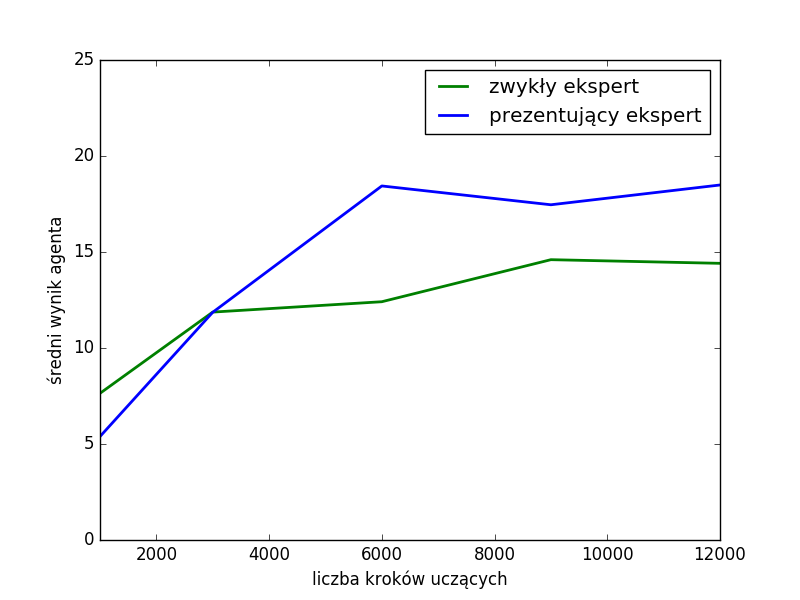
\includegraphics[scale = 0.7]{figures/figures/results/comp_dtc_plot.png}}{\caption{Porównanie wyników poszczególnych metod dla scenariusza \textit{Obrona środka}}\label{fig:dtc_comparison}}
\end{figure}

Z ostatecznego porównania wykluczono metodę \textit{agregacji zbioru danych} ponieważ, jak wspomniano w dedykowanym jej podrozdziale, agent uzyskany za pomocą \textit{świadomie prezentującego eksperta} nie przejawia żadnych zachowań, które \textit{agregacja} miała poprawiać. Wstępne eksperymenty pokazywały też niezadawalające osiągi tej metody i problemy analogiczne jak dla scenariusza \textit{Trudne zbieranie apteczek}.


\subsubsection{Trudne zbieranie apteczek}

W tabeli \ref{tab:health_comparison} i na rysunku \ref{fig:health_comparison} przedstawiono porównanie wyników badanych metod z wynikami uzyskanymi przez autorów środowiska VizDoom za pomocą tradycyjnych metod uczenia ze wzmocnieniem.

\begin{figure}[H]
		\ffigbox{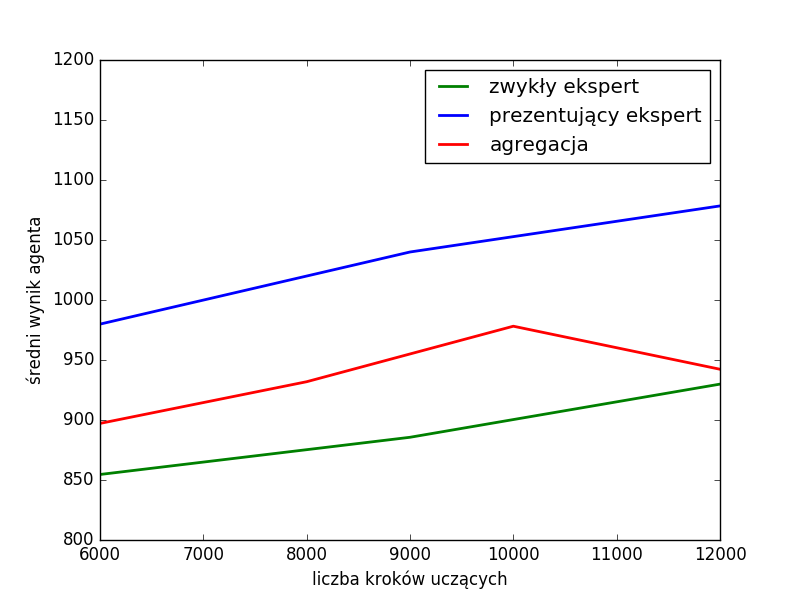
\includegraphics[scale = 0.7]{figures/figures/results/comp_hg_plot.png}}{\caption{Porównanie wyników poszczególnych metod dla scenariusza \textit{Trudne zbieranie apteczek}}\label{fig:health_comparison}}
\end{figure}

\textit{Prezentujący ekspert} występuje w zestawieniu trzykrotnie: pierwszy wpis traktuje metodę jako osobny i samodzielny przebieg. Kolejne wpisy zakładają, że najpierw konieczne było nauczenie agenta za pomocą \textit{zwykłego eksperta} (6000 kroków). Zachowanie takiego agenta zostało przeanalizowane, a następnie \textit{prezentujący ekspert} przeprowadził kolejną prezentację (6000 lub 12000 kroków) mając na uwadze błedy popełniane przez pierwszego agenta.

Najwyższy średni wynik, ze sporym zapasem, osiąga tradycyjny \textit{Q-learning}, zaimplementowany i zaprezentowany przez autorów pracy \cite{DBLP:journals/corr/KempkaWRTJ16}. Ta metoda jest jednak, jak wilokrotnie wspomniano wcześniej, bardzo wymagająca czasowo: ostateczny wynik uzyskany jest po 29 godzinach, a rezultaty porównywalne z badanymi w tej pracy osiągane są dopiero po około 9 godzinach nauki.

Spośród metod \textit{uczenia przez demonstację} wyraźną przewagę ma \textit{klonowanie zachowań ze świadomie prezentującym ekspertem}, a wygenerowane tym sposobem agenty zachowują się też najlepiej przy ocenie wizualnej. Metoda \textit{agregacji zbioru danych} ma średni wynik nieznacznie lepszy niż bazowe \textit{klonowanie zachowań}, ale ogromna wariancja uzyskiwanych wyników, jak i znacznie większe wykorzystanie eksperta stawia ją na ostatnim miejscu.

Żadnej z metod, łącznie z \textit{Q-learningiem} nie udało się wyeliminować największoego problemu z zachowaniem agenta, czyli wchodzenia w miny.

\subsection{Uczenie przez demonstację a Q-learning}

Jak wyraźnie widać w tabeli \ref{tab:health_comparison}, bezpośrednie porównywanie metod \textit{uczenia przez demonstację} z \textit{Q-learningiem} mija się z celem. \textit{Q-learning} osiąga wyraźnie lepsze wyniki, ale nauka za jego pomocą zajmuje ponad 100 razy więcej czasu. Oznacza to, że dla badanego problemu \textit{uczenie przez demonstację} spełniło swoje zadanie: pozwoliło wygenerować przyzwoicie zachowującego się agenta w ułamku czasu potrzebnego na nauczenie tradycyjnymi metodami uczenia ze wzmocnieniem jego odpowiednika.

Na szczególną uwagę zasługuje czas, jaki jest potrzebny na wytrenowanie agentów. Wykorzystanie 10 minut czasu eksperta pozwala zaoszczędzić 30 godzin czasu maszynowego nauki. Oczywiście, w niektórych przypadkach, przy wystarczających zasobach, 29 godziny automatycznej nauki może być korzystniejsze i tańsze niż wykorzystanie ludzkiego eksperta przez 10 minut. Trzeba jednak zauważyć, że wdrożenie każdego praktycznego zastosowanie wymaga wielu iteracji poprawek i konfiguracji. Przy wykorzystaniu \textit{uczenia przez demonstację} czas zbierania trajektorii eksperta jest jedno lub kilkurazowy. Na raz zebranych trajektoriach eksperta można wielokrotnie przeprowadzać relatwynie szybkie eksperymenty z wykorzystaniem innych parametrów i metod. W przypadku \textit{Q-learningu} każda zmiana wymaga każdorazowo wielu powtórzeń wielogodzinnych testów.

Z drugiej strony, zachowanie uzyskanych agentów wskazuje, że dalsze poprawianie ich za pomocą metod \textit{uczenia przez demonstację} może być trudne, a uzyskanie zauważlnie lepszych wyników niemożliwe. Przejawiane problemy, czyli przede wszystkim niedokładność agentów i wchodzenie w miny, powinny być dużo łatwiejsze do wyeliminowania z użyciem uczenia ze wzmocnieniem, dlatego obiecującym rozwiązaniem jest połączenie obu algorytmów, co udało się skutecznie zrobić autorom pracy \cite{DBLP:journals/corr/HesterVPLSPSDOA17}.


